\documentclass[border=10pt]{standalone}
\usepackage{forest}
\tikzset{
  tree node/.style = {align=center, inner sep=0pt, font = \scriptsize},
  S/.style = {draw, rectangle, minimum size = 8mm,  top color=white, bottom color=blue!20},
  tree node label/.style={font=\scriptsize},
}

\begin{document}

\newcommand{\tab}{\hspace{1cm}}
\newcommand{\taba}{\hspace{0.1cm}}

     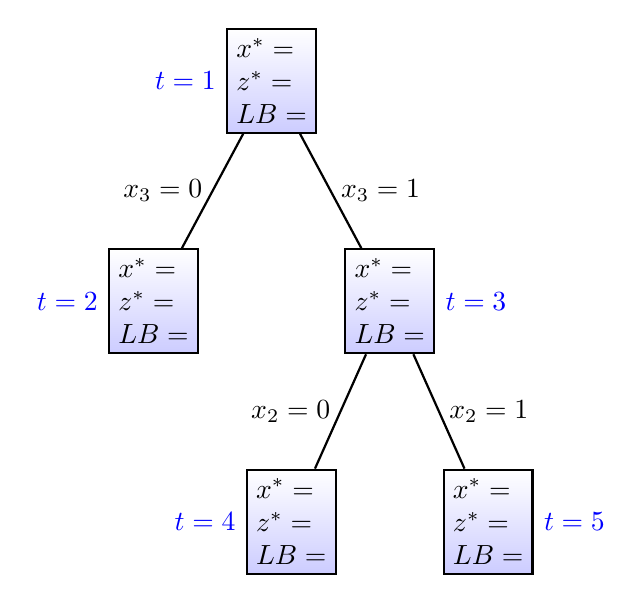
\begin{tikzpicture}[-,thick]
     
\node[S,sibling distance=3cm, level distance=1.3cm, align=left, label={[blue]left:$t = 1$}] 
	{$x^* = \tab $\\ $z^* = $\\ $ LB = $} 
	[sibling distance=3cm, level distance=2.8cm,align=left]
	%
     	child {node[S, label={[blue]left:$t = 2$}] 
     		{$x^* = \tab $\\$z^* = $\\$ LB = $}
		[sibling distance=2.5cm, level distance=2.8cm,align=left]
     		%child {node[S, label={[blue]above:$t = \tab$}] {$x^* = \tab$\\$z^* = $\\$ LB = $}
     			%edge from parent node[left] {help!}}
     		%child {node[S, label={[blue]above:\taba $t =$}] {$x^* = \tab$\\$z^* = $\\$ LB = $}
     			%edge from parent node[right] {help!}}
   		edge from parent node[left] {$x_3 = 0$}
   }
     child {node[S, label={[blue]right:\taba$t =3$}] 
     		{$x^* = \tab $\\$z^* = $\\$ LB = $}
		[sibling distance=2.5cm, level distance=2.8cm,align=left]
		%
     		child {node[S, label={[blue]left:$t = 4$}] {$x^* = \tab$\\$z^* = $\\$ LB = $}
     			edge from parent node[left] {$x_2 = 0$}}
     		child {node[S, label={[blue]right:$t =5$}] {$x^* = \tab$\\$z^* = $\\$ LB = $}
     			edge from parent node[right] {$x_2 = 1$}}
   		edge from parent node[right] {$x_3 = 1$}
   };

     \end{tikzpicture}



\end{document}